\begin{mdframed}[style=warning]
	\begin{ejercicio}
		\textbf{Conceptos.}
		\begin{enumerate}
			\item Suponga que usted atrapa una pelota de béisbol y, después, alguien le ofrece la opción de atrapar una bola para jugar a los bolos con el mismo momento lineal, o bien, con la misma energía cinética que la pelota. ¿Qué elegiría? ¿Por qué?

		\end{enumerate}
	\end{ejercicio}
\end{mdframed}











\begin{mdframed}[style=warning]
	\begin{ejercicio}
		Una masa $m_1$ con velocidad $v_o$, golpea un sistema masa resorte $m_2$ inicialmente en reposo. El resorte no tiene masa y tiene una constante $k$. No hay fricción. \\
		\begin{center}
			


\tikzset{every picture/.style={line width=0.75pt}} %set default line width to 0.75pt        

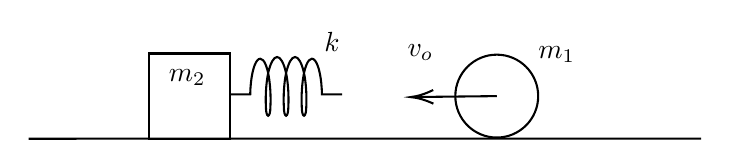
\begin{tikzpicture}[x=0.75pt,y=0.75pt,yscale=-1,xscale=1]
%uncomment if require: \path (0,307); %set diagram left start at 0, and has height of 307

%Straight Lines [id:da2006634064610846] 
\draw    (139,181) -- (463,180.94) ;
%Shape: Rectangle [id:dp9899626707813869] 
\draw   (197,139.94) -- (236,139.94) -- (236,181) -- (197,181) -- cycle ;
%Shape: Circle [id:dp16970128247733873] 
\draw   (344.54,160.47) .. controls (344.54,149.44) and (353.47,140.5) .. (364.5,140.5) .. controls (375.53,140.5) and (384.46,149.44) .. (384.46,160.47) .. controls (384.46,171.5) and (375.53,180.43) .. (364.5,180.43) .. controls (353.47,180.43) and (344.54,171.5) .. (344.54,160.47) -- cycle ;
%Shape: Inductor (Air Core) [id:dp8465340354701729] 
\draw   (236,159.65) -- (245.72,159.65) .. controls (245.86,152.05) and (247.21,145.55) .. (249.12,143.28) .. controls (251.03,141.01) and (253.11,143.43) .. (254.36,149.37) .. controls (255.32,154.01) and (255.72,160) .. (255.44,165.82) .. controls (255.44,168.09) and (254.96,169.94) .. (254.36,169.94) .. controls (253.76,169.94) and (253.28,168.09) .. (253.28,165.82) .. controls (253,160) and (253.4,154.01) .. (254.36,149.37) .. controls (255.48,144.43) and (257.04,141.63) .. (258.68,141.63) .. controls (260.32,141.63) and (261.88,144.43) .. (263,149.37) .. controls (263.96,154.01) and (264.36,160) .. (264.08,165.82) .. controls (264.08,168.09) and (263.6,169.94) .. (263,169.94) .. controls (262.4,169.94) and (261.92,168.09) .. (261.92,165.82) .. controls (261.64,160) and (262.04,154.01) .. (263,149.37) .. controls (264.12,144.43) and (265.68,141.63) .. (267.32,141.63) .. controls (268.96,141.63) and (270.52,144.43) .. (271.64,149.37) .. controls (272.6,154.01) and (273,160) .. (272.72,165.82) .. controls (272.72,168.09) and (272.24,169.94) .. (271.64,169.94) .. controls (271.04,169.94) and (270.56,168.09) .. (270.56,165.82) .. controls (270.28,160) and (270.68,154.01) .. (271.64,149.37) .. controls (272.89,143.43) and (274.97,141.01) .. (276.88,143.28) .. controls (278.79,145.55) and (280.14,152.05) .. (280.28,159.65) -- (290,159.65) ;
%Straight Lines [id:da31240970597204387] 
\draw    (364.5,160.47) -- (325,160.91) ;
\draw [shift={(323,160.94)}, rotate = 359.35] [color={rgb, 255:red, 0; green, 0; blue, 0 }  ][line width=0.75]    (10.93,-3.29) .. controls (6.95,-1.4) and (3.31,-0.3) .. (0,0) .. controls (3.31,0.3) and (6.95,1.4) .. (10.93,3.29)   ;

% Text Node
\draw (383,135) node [anchor=north west][inner sep=0.75pt]    {$m_{1}$};
% Text Node
\draw (205,146) node [anchor=north west][inner sep=0.75pt]    {$m_{2}$};
% Text Node
\draw (280,128) node [anchor=north west][inner sep=0.75pt]    {$k$};
% Text Node
\draw (320,134) node [anchor=north west][inner sep=0.75pt]    {$v_{o}$};


\end{tikzpicture}

		\end{center}
		¿Cuál es la máxima compresión del resorte?
	\end{ejercicio}
\end{mdframed}












\begin{mdframed}[style=warning]
	\begin{ejercicio}
		Se tiene una bola de masa $M$ a una altura $h$ y una pelotita de masa $m$ se encuentra arriba de la bola una distancia muy pequeña. El sistema se libera, encuentre $\flatfrac{M}{m}$ de modo que se de la máxima transferencia de energía. (Suponga choques elásticos)
	\end{ejercicio}
\end{mdframed}


































































































%%%